% !TeX spellcheck = es_ES
%%%%%%%%%%%%%%%%%%%%%%%%%%%%%%%%%%%%%%%%%
% Stylish Article
% LaTeX Template
% Version 2.1 (1/10/15)
%
% This template has been downloaded from:
% http://www.LaTeXTemplates.com
%
% Original author:
% Mathias Legrand (legrand.mathias@gmail.com) 
% With extensive modifications by:
% Vel (vel@latextemplates.com)
% Final ACS by:
% Juan Barbosa
% License:
% CC BY-NC-SA 3.0 (http://creativecommons.org/licenses/by-nc-sa/3.0/)
%
%%%%%%%%%%%%%%%%%%%%%%%%%%%%%%%%%%%%%%%%%
\documentclass[fleqn,10pt]{SelfArx}
%\usepackage[superscript]{cite}
\usepackage{wrapfig}
\usepackage{multirow}
%----------------------------------------------------------------------------------------
%	ARTICLE INFORMATION
%----------------------------------------------------------------------------------------

\JournalInfo{Laboratorio de Bioquímica, 07/02/2019} % Journal information
\Archive{ }

\PaperTitle{Aislamiento y determinación de ácidos nucleicos} %
%\Keywords{Keyword1 --- Keyword2 --- Keyword3} % Keywords - if you don't want any simply remove all the text between the curly brackets
%\newcommand{\keywordname}{Keywords} % Defines the keywords heading name

%----------------------------------------------------------------------------------------
%	ABSTRACT
%----------------------------------------------------------------------------------------

\Abstract{
}

%----------------------------------------------------------------------------------------

\begin{document}

\flushbottom % Makes all text pages the same height

\maketitle % Print the title and abstract box
%\tableofcontents % Print the contents section

\thispagestyle{empty} % Removes page numbering from the first page



%----------------------------------------------------------------------------------------
%	ARTICLE CONTENTS
%----------------------------------------------------------------------------------------

\section*{Introducci\'on} % The \section*{} command stops section numbering
%------------------------------------------------
	
\section{Secci\'on experimental}
	
\section{Resultados y Discusi\'on}
	\subsection{Aislamiento del ARN de levadura}
		Al disolver la levadura comercial en agua a una temperatura de 37 $^\circ$C se busca activar el metabolismo del hongo, para que esto pueda suceda es necesario que el organismo produzca ARN con el fin de iniciar la producci\'on de prote\'inas. En este sentido el control de la temperatura debe ser estricto, dado que cambios aumentos abruptos en esta, pueden llevar a que el organismo muera y cese su producci\'on del ARN que posteriormente ser\'a cuantificado.
		
		La adici\'on de fenol permite extraer los \'acidos nucleicos de la levadura dada la polaridad del mismo. Los \'acidos nucleicos debido a sus grupos fosfatos, constituyen mol\'eculas polares, las cuales se disuelven mejor en agua que en fenol. El proceso contrario sucede con las prote\'inas, las cuales tender\'an a estar en la fase org\'anica. La centrifugaci\'on de esta mezcla permite realizar la separaci\'on de fases, en donde en la fase acuosa se obtienen mayormente \'acidos nucleicos y prote\'inas desnaturalizadas. La siguiente centrifugaci\'on permite aislar los \'acidos nucleicos de las prote\'inas desnaturalizadas.
		
		Finalmente, y con el objetivo de precipitar los \'acidos nucleicos se adiciona acetato de potasio y etanol, los cuales promueven la formaci\'on de enlaces entre los aniones de los grupos fosfatos de los \'acidos nucleicos, y el ion potasio, con lo cual se neutraliza la mol\'ecula, ocasionando su precipitaci\'on.
		
		
%		 If the aim of an experiment is to obtain samples of purified RNA, a pH of around 4.5 is used. Because of the negative charge on the backbone of DNA from phosphates, decreasing the pH of a solution will lead to neutralization. A pH of 4.5 has a higher concentration of H+ ions that would neutralize the negative phosphate charges and cause DNA to dissolve in the organic phase, while RNA has additional hydroxyl group in pentose sugar which allows the RNA to remain in water phase. 
%		\cite{toni2018optimization}
		
	\subsection{Aislamiento del ADN de fresa}
		Para extraer el ADN de la \textit{F. ananassa}, se hace uso de detergente, el cual tiene como objetivo disolver las membranas de las células, en un proceso conocido como lisis \cite{virgili2006genoma, puerta2005practicas}. Al disolver las proteínas se interrumpen las interacciones de la bicapa lipídica: proteína-proteína, lípido-lípido y lípido-proteína. La adición de cloruro de sodio junto con la bromelina de la piña, permite desnaturalizar y clivar las proteínas estructurales del ADN, las cuales reciben el nombre de histonas \cite{poh2011thermal}. Posteriormente y dado que los ácidos nucleicos no son solubles en alcoholes, con la adición de etanol frío, se obtiene el ADN en suspensión.
		
		La justificación del uso de la fresa se debe a que esta presenta poliploidia, es decir existen variedades octaploides y diploides, esto a su vez significa que algunas de ellas cuentan con ocho copias de su genoma, garantizando una alta disponibilidad de material genético para su extracción \cite{husaini2016strawberry}.
	
	\subsection{Aislamiento de ADN genómico de bacterias}
		En el caso de las bacterias, la extracción del ADN se realiza usando una desnaturalización térmica a temperatura de ebullición, de las histonas.
	
	\subsection{Cuantificaci\'on de \'acidos nucleicos}
		Una de las formas más usadas actualmente para determinar de forma rápida la cantidad y pureza de los ácidos nucleicos es usando espectroscopía UV-vis. En el rango de longitudes de onda de 215 a 230 nm se encuentra la absorción de los enlaces peptídicos, un poco debajo de 260 nm se encuentra la absorción de las purinas, mientras que las pirimidinas absorben arriba de 260 nm, siendo ambas las bases nitrogenadas constituyentes de los ácidos nucleicos. Finalmente en 280 nm se encuentran las absorciones de los aminoácidos aromáticos \cite{sambrook2001molecular}.
		
	\begin{figure*}[h]
		\centering
		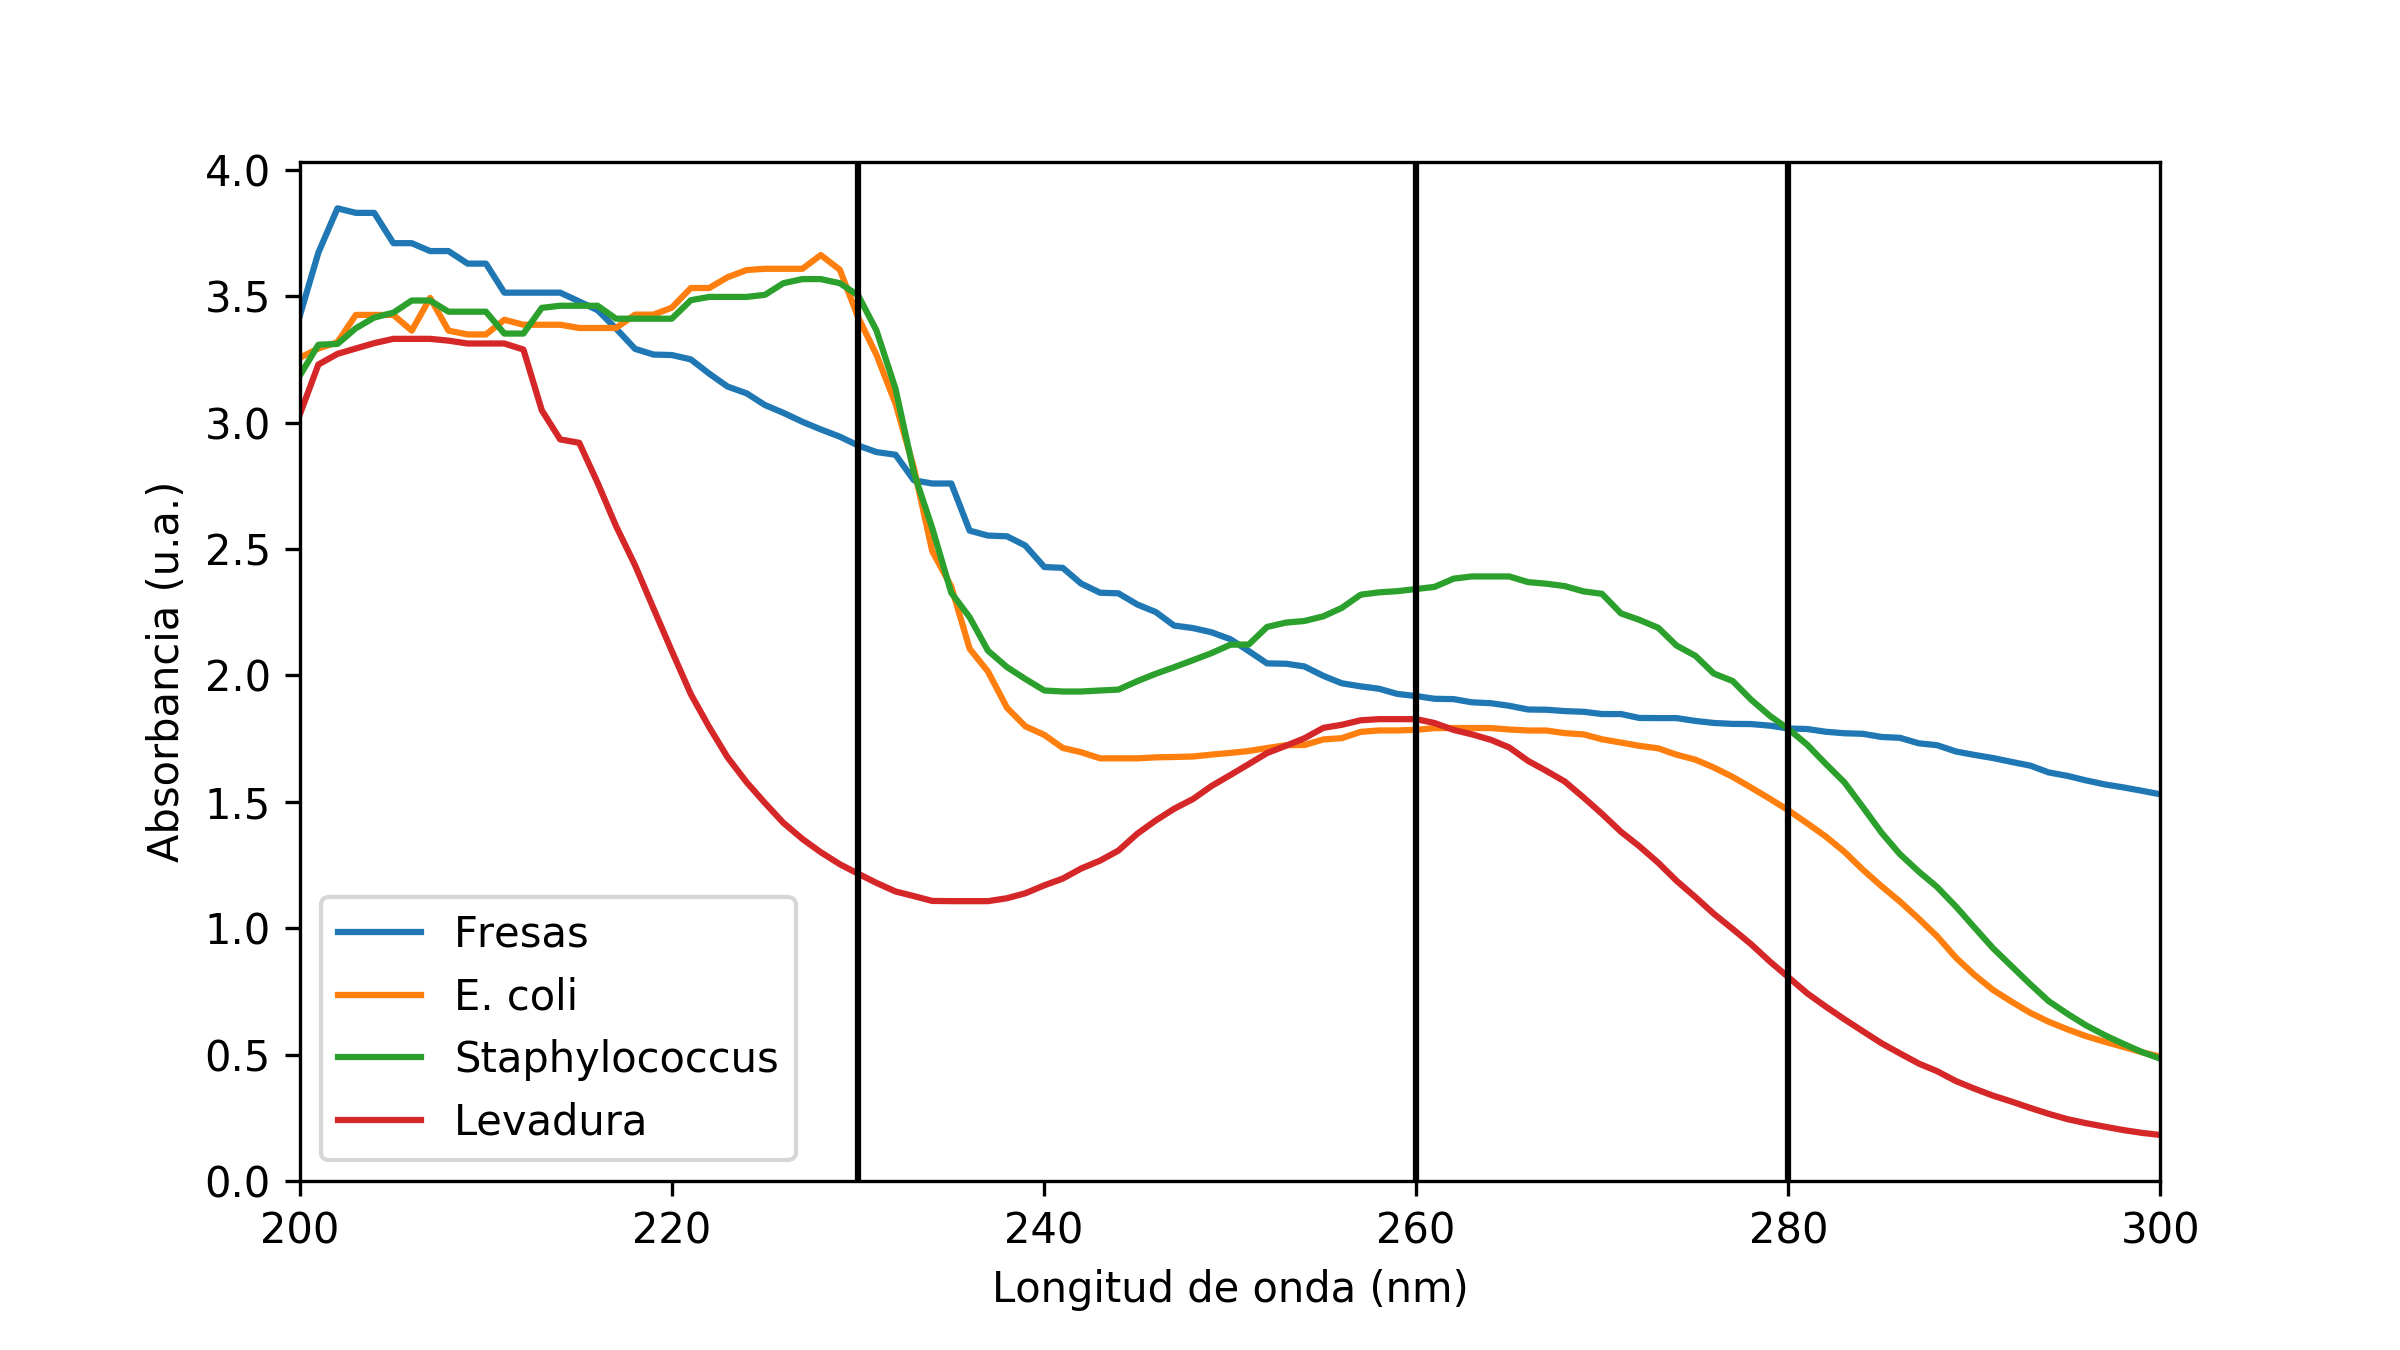
\includegraphics[width=\linewidth]{plots}
		\caption{Absorbancias obtenidas para las distintas muestras en funci\'on de la longitud de onda.}
		\label{fig}
	\end{figure*}	

	\begin{table}[h]
		\centering
		\caption{Absorbancias a 230, 260 y 280 nm (u.a.), junto con la relaci\'on 260/280.}
		\begin{tabular}{c|ccc|c}
			\hline
			\textbf{Muestra} & $A_{230}$ & $A_{260}$ & $A_{280}$ & $A_{260} / A_{280}$ \\
			\hline
			\textit{F. ananassa} & 2.97 & 1.91 & 1.79 & 1.06 \\
			\textit{E. coli} & 4.85 & 1.79 & 1.47 & 1.22 \\
			\textit{S. aureus} & 3.50 & 2.35 & 1.79 & 1.31 \\
			\textit{S. cerevisiae} & 1.22 & 1.83 & 0.81 & 2.27 \\
			\hline
		\end{tabular}
		\label{tb}
	\end{table}

	En la \autoref{fig} se muestran los espectros de absorción obtenidos para las cuatro muestras analizadas, en donde las bandas grises muestran las longitudes de onda de interés. Adicionalmente, en la \autoref{tb} se tienen las absorbancias para 230, 260 y 280 nm. A partir de la información obtenida en 230 nm, que la muestra de ácidos nucleicos de mayor pureza es la de \textit{S.cerevisiae}, pues la concentración de enlaces peptídicos es cerca de 3 veces inferior a las demás.

	El análisis para la fresa no arrojó resultados concluyentes, pues si bien es posible calcular el radio entre la absorción en 280 nm y 260 nm, en la \autoref{fig} no se observa ninguna banda en todo el espectro por lo cual se considera que la información registrada corresponde en realidad a ruido producto de la concentración de la muestra. Para el ADN de las bacterias es posible comprobar la presencia de ADN y de proteínas, pues se espera que a mayor concentración de proteínas en la solución aumente la absorbancia en 280 nm, disminuyendo el valor de $A_{260} / A_{280}$. Esto además es confirmado al considerar la absorción a 230 nm, la cual es considerablemente alta, mostrando que si bien la extracción del ADN fue exitosa en ambas bacterias, la separación de los ácidos nucleicos y las proteínas no fue idónea.
	
	Finalmente, para la muestra de ARN de \textit{S. cerevisiae} se obtuvieron los mejores resultados, a pesar que se registró un valor superior a 2 para la relación $A_{260} / A_{280}$, se debe tener en cuenta un contaminante com\'un que puede aumentar las lecturas de absorbancia en 260 nm es el fenol, el cual absorbe en 270 nm y pudo haber permanecido en la muestra luego del proceso de extracci\'on \cite{toni2018optimization}.
	
	Respecto a la recuperación de ADN de \textit{F. ananassa} se obtuvieron cerca de 0.6342 g para una fresa, mientras que para 2.5 g de \textit{S. cerevisiae} la recuperación fue de 0.3471 g. Considerando una cuota superior para la concentración, dada por ADN puro, de doble hélice se tiene que 50 $\mu$g/mL equivalen a 1 unidad de absorbancia \cite{sambrook2001molecular}. De esta forma se estima que la concentración en la solución medida para \textit{E. coli} es 89.5 $\mu$g/mL, y para \textit{S. aureus} es 117.5 $\mu$g/mL. Para el ARN la extinción es de 40 $\mu$g/mL a 260 nm, con lo cual se obtiene para \textit{S. cerevisiae} una concentración de 73.2 $\mu$g/mL.
	
\section{Conclusiones}
	Fue posible determinar la presencia de ácidos nucleicos en muestras biológicas: vegetales, fúngicas y bacterianas, usando espectroscopia UV-vis. La pureza del ADN para las muestras de bacterias \textit{E. coli} y \textit{S. aureus} y el ARN de	\textit{S. cerevisiae} fue discutida teniendo en cuenta las absorciones a 230, 260 y 280 nm, encontrando una correlación entre la absorbancia de los aminoácidos aromáticos y los enlaces peptídicos para las primeras dos, y un pequeño aumento en el valor esperado de 2 para la relación $A_{260} / A_{280}$ en el caso del hongo. Una cuota superior para las concentraciones de ácidos nucleicos fue establecida para cada una de estas tres especies: 89.5, 117.5 y 73.2 $\mu$g/mL, correspondientemente. Finalmente, cada uno de los pasos involucrados en el aislamiento de la información genética de cada muestra fue analizado en detalle, destacando el papel de cada uno de los reactivos adicionados.
	
%----------------------------------------------------------------------------------------
%	REFERENCE LIST
%----------------------------------------------------------------------------------------
\phantomsection
\bibliography{informe}
\bibliographystyle{unsrt}

%----------------------------------------------------------------------------------------
%\newpage
%\onecolumn
%\section{Informaci\'on suplementaria}\label{sec: complementaria}
\end{document}